% Pursuing Stacks (cotes 134-2 to 134-8): archive cote 134-3, site page 69 (PDF page 70), typescript page 69.
% typescript. Draft compared: ps2.tex:3564-3633.
% AI-transcribed by Claude Opus 5.5 (claude-opus-5-5, adaptive thinking, effort high), Message Batches API, batch ps1 (msgbatch_01Rv5hCaNTtUt4JHx1yqoHPL), 2026-11-12; image review recorded in records/CHECK_DECISIONS_134_3_4.tsv.
\scanpage{134-3/69}
\mspage{\hand{69}}
sian powers of I, plus products $a_{o}xI^{n}$ $(n\hand{\in}\underline{N})$ \over{a}{,} where $a_{o}$ is an extra element\hand{,}
and \inserted{as} maps between these all those (and not more) which can be deduced from
$\hand{\delta}_{o},\hand{\delta}_{1}$ and the assumption that the elements $I^{n}$ and $axI^{n}$ are cartesian pro-%
ducts indeed. This is much in the spirit of the construction of a variant
of the category \hand{\ensuremath{\square}} of ``standar\over{t}{d} cubes'', \over[typed]{what}{which} naturally came to mind
a while ago (cf p. 48-49). I very much doubt A satisfies T 2), and would
rather bet that $a_{o}xa_{o}$ in $A^{\hand{\wedge}}$is \uline{not} aspheric.

Another type of example comes to my mind, starting with a perfectly
good \hand{(}namely \uline{strict}\hand{)} test category A, and taking an induced category
$A_{/a_{o}}$ , with $a_{o}$ in A. This is of course a \over[typed]{t}{t}est category (it would have been
enough that A be just a local test category\hand{)}, however it is unlikely that
it will satisfy T\over[typed]{a}{2} namely the induced topos be totally aspheric. This
w\over{ill}{ould} imply for instance that for any two \xout{subob} non empty subobjects of
$a_{o}$ in $A^{\hand{\wedge}}$ (namely subobjects of the final element in $A^{\hand{\wedge}}_{/a_{o}}$ \hand{\ensuremath{\simeq}} $(A_{/a_{o}})^{\hand{\wedge}}$) h\over[typed]{\unsure{q}}{a}\over[typed]{t}{v}e a
non empty intersection. Now this is an exceedingly strong property of $a_{o}$ ,
which is practically never satisfied, except for the final object of A.
N\over[typed]{e}{o}w here is a kind of ``universal'' coun\over[typed]{t}{t}erexample. Take A any \over[typed]{t}{t}est category
and I a homotopy interval in $A^{\hand{\wedge}}$, thus I is aspheric and hence $A_{/I}$ is
again a test category (namely locally test and aspheric), but it is \uline{never}
a strict test category, because the two standart subobjects $e_{o},e_{1}$ given
with the structure of I are non-empty, and however their intersection is
\margin{\diagram{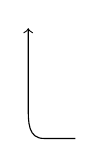
\begin{tikzpicture}\draw[->] (.6,0)--(.2,0) .. controls (0,0) and (0,.2) .. (0,.4)--(0,1.4);\end{tikzpicture}}}empty !

These reflections bring very near how much stronger the \inserted{extra} strictness
requi\over[typed]{\unsure{t}}{r}ement T 2 for test categories, than merely the conditions T 1, T3
without T 2 .

40. Yesterday I incidentally made use of the fact that if A is an asphe-%
ric element in (Cat), th\over[typed]{\unsure{a}}{e}n for any other object C, CxA \hand{\ensuremath{\longrightarrow}} C is aspheric
(and a fortiori a weak equivalence). The usual asphericity criterion for a
functor shows that it is enough to prove that for any C with final element,
\margin{\diagram{\begin{tikzpicture}\draw[->] (.6,1.4)--(.2,1.4) .. controls (0,1.4) and (0,1.2) .. (0,1)--(0,0);\end{tikzpicture}}}CxA is aspheric. \xout{Thusxw} For this again it is enough to prove that the
projection CxA \hand{\ensuremath{\longrightarrow}} A is aspheric, which by localisation up\over[typed]{n}{o}n A means that
the product categories \hand{.} Cx\hand{(}$A_{/a}$\hand{)} (with a in A) are aspheric. Finall\over{\unsure{x}}{y} we
are reduced to checking that the product of two categories with final ele-%
ment is aspheric, which is trivial because such a category has itself a
final element.

The result just proved can be viewed as a particular case of the
following
\uline{Proposition} In (Cat), the cartesian product of two weak equivalences is
a weak equivalence.
